\documentclass[style=sailor,size=12pt]{powerdot}
\usepackage{epic,array,ecltree,url,calrsfs}
\usepackage[nointegrals]{wasysym}
\usepackage{listings}
\usepackage{epsfig}
\usepackage{amsmath}
\usepackage{amsfonts}
\usepackage{amssymb}
\usepackage{amsxtra}
\usepackage{amsthm}
\usepackage{mlextra} % Must be below ams packages
\usepackage{mathrsfs}
\usepackage{color}
\usepackage{array}
\usepackage{graphicx}
\graphicspath{ {../art/} }
\usepackage{bm}
\usepackage{tikz}
\usepackage{multicol}
\usepackage{enumitem}
\usepackage{blkarray}
\usepackage{bigstrut}
\setlength{\bigstrutjot}{4pt}
\usetikzlibrary{arrows}
\usepackage{subcaption}

\pdsetup{method=normal}

\title{Review: Relations and Functions}
\author{Foundations of Computer Science}
\date{\today}

\begin{document}
\maketitle
\section[slide=true]{Relations}
\begin{slide}[bm=,toc=]{Definition}
\begin{defn}{A.19}[Ben Ari]
An \emph{n-ary relation} $\mathcal{R}$ is a subset of $S_1 \times \cdots \times
S_n$. 
\begin{itemize}
\item $\mathcal{R}$ is said to be a relation \emph{on} $S_1 \times \cdots \times
S_n$.
\item If all the sets $S_i$ are the same set $S$, $\mathcal{R}$ is said to be
an \emph{n-ary} relation on $S$.
\item A 1-ary (unary) relation is simply a subset.
\end{itemize}
\end{defn}
\end{slide}

\begin{slide}[bm=,toc=]{Examples of Binary Relations}
\begin{ex}{}[Explicit]~\\
\begin{itemize}
\item Let $L = \{a,b,c\}$.
\item Let $W = \{all,ball,bat,cat\}$.
\item The we can define binary relation $R \subseteq L \times W$ such that 
      $R = \{(a,all),(b,ball),(b, bat), (c,cat)\}$.
\end{itemize}
\end{ex}
\begin{ex}{}[Set Comprehension]~\\
\begin{itemize}
\item Let $\Sigma = \{a,b\}$.
\item Let $S = \Sigma^0 \cup \Sigma \cup \Sigma^2$
\item Define binary relation $R_{pre}$ on $S$ such that:
      $R_{pre} = \{(x,y)| y = xw \text{ for some } w \in S \}$.
\end{itemize}
\end{ex}

\end{slide}

\begin{slide}[bm=,toc=]{Matrix Representations of Relations}
Relations can be represented using a binary matrix in which the
value corresponding to a tuple is set to $1$ if the tuple is
in the relation, and $0$ otherwise.
\begin{ex}{}[$R$ and $R_{pre}$ from previous slide]
\[
R = 
\begin{blockarray}{cccc}
\begin{block}{cccc}
& a & b & c \\
\end{block}
\begin{block}{c[ccc]}
all  & 1 & 0 & 0 \bigstrut[t] \\
ball & 0 & 1 & 0 \\
bat  & 0 & 1 & 0 \\
cat  & 0 & 0 & 1 \\
\end{block}
\end{blockarray}
\qquad R_{pre} =
\begin{blockarray}{cccccccc}
\begin{block}{cccccccc}
 & \epsilon & a & b & aa & ab & ba & bb \\
\end{block}
\begin{block}{c[ccccccc]}
\epsilon & 1  & 1 & 1 & 1  & 1  & 1  & 1\bigstrut[t] \\
a  & 0& 1 & 0 & 1  & 1  & 0  & 0 \\
b  & 0& 0 & 1 & 0  & 0  & 1  & 1 \\
aa & 0& 0 & 0 & 1  & 0  & 0  & 0 \\
ab & 0& 0 & 0 & 0  & 1  & 0  & 0 \\
ba & 0& 0 & 0 & 0  & 0  & 1  & 0 \\
bb & 0& 0 & 0 & 0  & 0  & 0  & 1 \\
\end{block}
\end{blockarray}
\]
\end{ex}
\end{slide}

\begin{slide}[bm=,toc=]{DiGraph Representations of Relations}
Binary relations can also be represented using a directed graph in which
vertices represent elements and edges are placed between vertices
if their corresponding tuple is in the relation.
\begin{ex}{}[$R$ and $R_{pre}$ from previous slide]
~\\
\vspace{-2mm}
\begin{figure}[h!]
\centering
\subcaptionbox*{$R$}[.3\linewidth]{
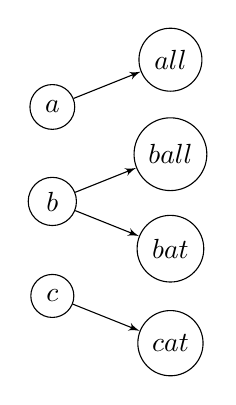
\begin{tikzpicture}
\tikzset{vertex/.style = {shape=circle,draw,minimum size=1.5em}}
\tikzset{edge/.style = {->,> = latex'}}

\node[vertex](c1) at (0,0.6) {$c$};
\node[vertex](b1) at (0,1.8) {$b$};
\node[vertex](a1) at (0,3) {$a$};
\node[vertex](d2) at (1.5,0) {$cat$};
\node[vertex](c2) at (1.5,1.2) {$bat$};
\node[vertex](b2) at (1.5,2.4) {$ball$};
\node[vertex](a2) at (1.5,3.6) {$all$};

\draw[edge] (a1) to (a2);
\draw[edge] (b1) to (b2);
\draw[edge] (b1) to (c2);
\draw[edge] (c1) to (d2);
\end{tikzpicture}
}
\subcaptionbox*{$R_{pre}$}[.5\linewidth]{
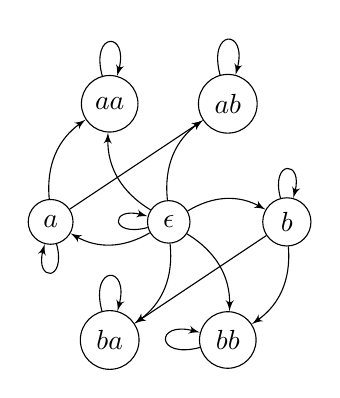
\begin{tikzpicture}
\tikzset{vertex/.style = {shape=circle,draw,minimum size=1.5em}}
\tikzset{edge/.style = {->,> = latex'}}

\node[vertex](aa) at (0.75,3) {$aa$};
\node[vertex](ab) at (2.25,3) {$ab$};
\node[vertex](a) at (0,1.5) {$a$};
\node[vertex](e) at (1.5,1.5) {$\epsilon$};
\node[vertex](b) at (3,1.5) {$b$};
\node[vertex](ba) at (0.75,0) {$ba$};
\node[vertex](bb) at (2.25,0) {$bb$};

\draw[edge] (a) to[loop below] (a);
\draw[edge] (b) to[loop above] (b);
\draw[edge] (e) to[loop left] (e);
\draw[edge] (aa) to[loop above] (aa);
\draw[edge] (ab) to[loop above] (ab);
\draw[edge] (ba) to[loop above] (ba);
\draw[edge] (bb) to[loop left] (bb);
\draw[edge] (e) to[bend left] (a);
\draw[edge] (e) to[bend left] (b);
\draw[edge] (e) to[bend left] (aa);
\draw[edge] (e) to[bend left] (ab);
\draw[edge] (e) to[bend left] (ba);
\draw[edge] (e) to[bend left] (bb);
\draw[edge] (a) to[bend left] (aa);
\draw[edge] (a) to (ab);
\draw[edge] (b) to (ba);
\draw[edge] (b) to[bend left] (bb);
\end{tikzpicture}
}
\end{figure}

\end{ex}
\end{slide}


\begin{slide}[bm=,toc=]{Reflexive Relations}
\begin{defn}{A.21}[Ben Ari]
Let $R$ be a binary relation on $S$.
\\~\\
$R$ is \emph{reflexive} if and only if $R(x,x)$ for all $x \in S$.
\end{defn}
~
\vspace{-12mm}
\pause \begin{figure}[t]
\caption*{\textbf{Example:} $R_{pre}$ is a reflexive relation on $S = \{\epsilon,a,b,aa,bb\}$} 
\pause \subcaptionbox*{As Matrix}{
$ \begin{blockarray}{cccccc}
 \begin{block}{cccccc}
  & \epsilon & a & b & aa & bb \\
 \end{block}
 \begin{block}{c[ccccc]}
 \epsilon & 1 & 1 & 1 & 1 & 1 \bigstrut[t] \\
 a        & 0 & 1 & 0 & 1 & 0  \\
 b        & 0 & 0 & 1 & 0 & 1  \\
 aa       & 0 & 0 & 0 & 1 & 0  \\
 bb       & 0 & 0 & 0 & 0 & 1  \\
 \end{block}
 \end{blockarray} $
}
\qquad
\pause \subcaptionbox*{As Digraph}{
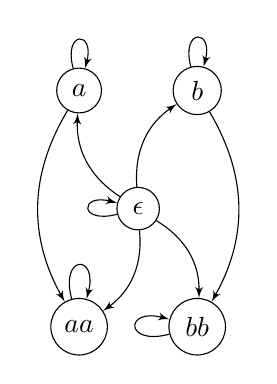
\begin{tikzpicture}
\tikzset{vertex/.style = {shape=circle,draw,minimum size=1.5em}}
\tikzset{edge/.style = {->,> = latex'}}

\node[vertex](a) at (0.75,3) {$a$};
\node[vertex](b) at (2.25,3) {$b$};
\node[vertex](e) at (1.5,1.5) {$\epsilon$};
\node[vertex](aa) at (0.75,0) {$aa$};
\node[vertex](bb) at (2.25,0) {$bb$};

\draw[edge] (a) to[loop above] (a);
\draw[edge] (b) to[loop above] (b);
\draw[edge] (e) to[loop left] (e);
\draw[edge] (aa) to[loop above] (aa);
\draw[edge] (bb) to[loop left] (bb);
\draw[edge] (e) to[bend left] (a);
\draw[edge] (e) to[bend left] (b);
\draw[edge] (e) to[bend left] (aa);
\draw[edge] (e) to[bend left] (bb);
\draw[edge] (a) to[bend right] (aa);
\draw[edge] (b) to[bend left] (bb);
\end{tikzpicture}
}
\end{figure}

\end{slide}

\begin{slide}[bm=,toc=]{Symmetric Relations}
\begin{defn}{A.21}[Ben Ari]
Let $R$ be a binary relation on $S$.
\\~\\
$R$ is \emph{symmetric} if and only if $R(x_1,x_2)$ implies $R(x_2,x_1)$.
\end{defn}
~
\vspace{-12mm}
\pause \begin{figure}[t]
\caption*{\textbf{Example:} $R_l$ is a symmetric relation on $S = \{\epsilon,a,b,aa,bb\}$} 
\pause \subcaptionbox*{As Matrix}{
$ \begin{blockarray}{cccccc}
 \begin{block}{cccccc}
  & \epsilon & a & b & aa & bb \\
 \end{block}
 \begin{block}{c[ccccc]}
 \epsilon & 1 & 0 & 0 & 0 & 0 \bigstrut[t] \\
 a        & 0 & 1 & 1 & 0 & 0  \\
 b        & 0 & 1 & 1 & 0 & 0  \\
 aa       & 0 & 0 & 0 & 1 & 1  \\
 bb       & 0 & 0 & 0 & 1 & 1  \\
 \end{block}
 \end{blockarray} $
}
\qquad
\pause \subcaptionbox*{As Digraph}{
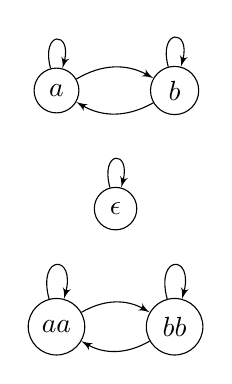
\begin{tikzpicture}
\tikzset{vertex/.style = {shape=circle,draw,minimum size=1.5em}}
\tikzset{edge/.style = {->,> = latex'}}

\node[vertex](a) at (0.75,3) {$a$};
\node[vertex](b) at (2.25,3) {$b$};
\node[vertex](e) at (1.5,1.5) {$\epsilon$};
\node[vertex](aa) at (0.75,0) {$aa$};
\node[vertex](bb) at (2.25,0) {$bb$};

\draw[edge] (a) to[loop above] (a);
\draw[edge] (b) to[loop above] (b);
\draw[edge] (e) to[loop above] (e);
\draw[edge] (aa) to[loop above] (aa);
\draw[edge] (bb) to[loop above] (bb);
\draw[edge] (a) to[bend left] (b);
\draw[edge] (b) to[bend left] (a);
\draw[edge] (bb) to[bend left] (aa);
\draw[edge] (aa) to[bend left] (bb);
\end{tikzpicture}
}
\end{figure}
\pause {\footnotesize Exercise: Give a rule for the relation.} 
\pause {\footnotesize \textbf{Ans:} $R_{l} = \{(x,y)| |x| = |y|\}$}
\end{slide}

\begin{slide}[bm=,toc=]{Antisymmetric Relations}
\begin{defn}{A.21}[Ben Ari]
Let $R$ be a binary relation on $S$.
\\~\\
$R$ is \emph{antisymmetric} if and only if $(x_1,x_2) \in R$ and $(x_2,x_1) \in
R$ implies $x_1 = x_2$.
\end{defn}
~
\vspace{-12mm}
\pause \begin{figure}[t]
\caption*{\textbf{Example:} $R_{pre}$ is also antisymmetric on $S = \{\epsilon,a,b,aa,bb\}$} 
\subcaptionbox*{As Matrix}{
$ \begin{blockarray}{cccccc}
 \begin{block}{cccccc}
  & \epsilon & a & b & aa & bb \\
 \end{block}
 \begin{block}{c[ccccc]}
 \epsilon & 1 & 1 & 1 & 1 & 1 \bigstrut[t] \\
 a        & 0 & 1 & 0 & 1 & 0  \\
 b        & 0 & 0 & 1 & 0 & 1  \\
 aa       & 0 & 0 & 0 & 1 & 0  \\
 bb       & 0 & 0 & 0 & 0 & 1  \\
 \end{block}
 \end{blockarray} $
}
\qquad
\subcaptionbox*{As Digraph}{
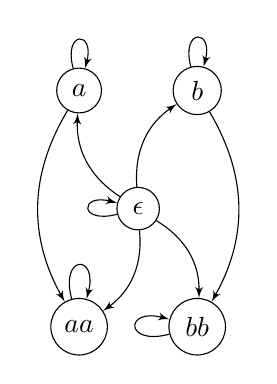
\begin{tikzpicture}
\tikzset{vertex/.style = {shape=circle,draw,minimum size=1.5em}}
\tikzset{edge/.style = {->,> = latex'}}

\node[vertex](a) at (0.75,3) {$a$};
\node[vertex](b) at (2.25,3) {$b$};
\node[vertex](e) at (1.5,1.5) {$\epsilon$};
\node[vertex](aa) at (0.75,0) {$aa$};
\node[vertex](bb) at (2.25,0) {$bb$};

\draw[edge] (a) to[loop above] (a);
\draw[edge] (b) to[loop above] (b);
\draw[edge] (e) to[loop left] (e);
\draw[edge] (aa) to[loop above] (aa);
\draw[edge] (bb) to[loop left] (bb);
\draw[edge] (e) to[bend left] (a);
\draw[edge] (e) to[bend left] (b);
\draw[edge] (e) to[bend left] (aa);
\draw[edge] (e) to[bend left] (bb);
\draw[edge] (a) to[bend right] (aa);
\draw[edge] (b) to[bend left] (bb);
\end{tikzpicture}
}
\end{figure}
\end{slide}

\begin{slide}[bm=,toc=]{Transitive Relations}
\begin{defn}{A.21}[Ben Ari]
Let $R$ be a binary relation on $S$.
\\~\\
$R$ is \emph{transitive} if and only if $R(x_1,x_2)$ and $R(x_2,x_3)$ implies $R(x_1,x_3)$.
\end{defn}
~
\vspace{-12mm}
\pause \begin{figure}[t]
\caption*{\textbf{Example:} Both $R_{pre}$ and $R_l$ are transitive on $S = \{\epsilon,a,b,aa,bb\}$} 
\subcaptionbox*{$R_{pre}$}{
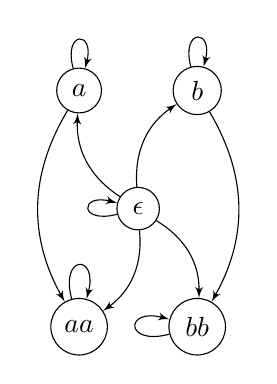
\begin{tikzpicture}
\tikzset{vertex/.style = {shape=circle,draw,minimum size=1.5em}}
\tikzset{edge/.style = {->,> = latex'}}

\node[vertex](a) at (0.75,3) {$a$};
\node[vertex](b) at (2.25,3) {$b$};
\node[vertex](e) at (1.5,1.5) {$\epsilon$};
\node[vertex](aa) at (0.75,0) {$aa$};
\node[vertex](bb) at (2.25,0) {$bb$};

\draw[edge] (a) to[loop above] (a);
\draw[edge] (b) to[loop above] (b);
\draw[edge] (e) to[loop left] (e);
\draw[edge] (aa) to[loop above] (aa);
\draw[edge] (bb) to[loop left] (bb);
\draw[edge] (e) to[bend left] (a);
\draw[edge] (e) to[bend left] (b);
\draw[edge] (e) to[bend left] (aa);
\draw[edge] (e) to[bend left] (bb);
\draw[edge] (a) to[bend right] (aa);
\draw[edge] (b) to[bend left] (bb);
\end{tikzpicture}
}
\qquad
\subcaptionbox*{$R_l$}{
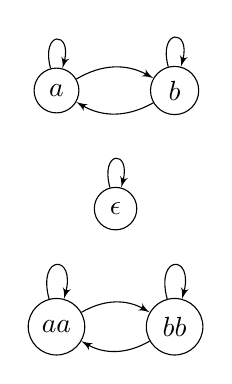
\begin{tikzpicture}
\tikzset{vertex/.style = {shape=circle,draw,minimum size=1.5em}}
\tikzset{edge/.style = {->,> = latex'}}

\node[vertex](a) at (0.75,3) {$a$};
\node[vertex](b) at (2.25,3) {$b$};
\node[vertex](e) at (1.5,1.5) {$\epsilon$};
\node[vertex](aa) at (0.75,0) {$aa$};
\node[vertex](bb) at (2.25,0) {$bb$};

\draw[edge] (a) to[loop above] (a);
\draw[edge] (b) to[loop above] (b);
\draw[edge] (e) to[loop above] (e);
\draw[edge] (aa) to[loop above] (aa);
\draw[edge] (bb) to[loop above] (bb);
\draw[edge] (a) to[bend left] (b);
\draw[edge] (b) to[bend left] (a);
\draw[edge] (bb) to[bend left] (aa);
\draw[edge] (aa) to[bend left] (bb);
\end{tikzpicture}
}
\end{figure}
\end{slide}
\begin{slide}[bm=,toc=]{Equivalence Relations}
\begin{defn}{--- Equivalence Relations}~\\
A relation is an equivalence relation if it is:

\begin{itemize}
\item Reflexive
\item Symmetric
\item Transitive
\end{itemize}
\end{defn}
\textbf{Examples}:
\begin{itemize}
\item $\{(x,y) | x = y \}$
\item $\{(x,y) | x \text{ and } y \text{ begin with the same character}\}$
\item $\{(x,y) | x \text{ and } y \text{ contain the same substring}\}$
\item $R_{l}$ 
\end{itemize}
\end{slide}

\begin{slide}[bm=,toc=]{Partial Orders}
\begin{defn}{--- Partial Orders}~\\
A relation is a partial order if it is:

\begin{itemize}
\item Reflexive
\item Antisymmetric
\item Transitive
\end{itemize}
\textbf{Examples}:
\begin{itemize}
\item $R_{pre}$
\item $\{(x,y) | x \text{ is a substring of } y \}$
\item $\{(x,y) | x \text{ is a subset of } y \}$
\item $\{(x,y) | y \text{ is a suffix of } x \}$
\end{itemize}
\end{defn}
\end{slide}

\begin{slide}[bm=,toc=]{Composition}
\end{slide}
\begin{slide}[bm=,toc=]{Powers}
\end{slide}

\section[slide=true]{Functions}
\begin{slide}[bm=,toc=]{Definition}
\begin{defn}{A.21}[Ben Ari]
Let $\mathcal{F}$ be a relation on $S_1 \times \cdots \times S_n$.
$\mathcal{F}$ is a \emph{function} iff for every \emph{$(n-1)$-tuple}
$(x_1,...,x_n) \in S_1 \times \cdots \times S_{n-1}$, there is at most
one $x_n \in S_n$, such that $\mathcal{F}(x_1,...,x_n)$.
\begin{itemize}
\item For a function $\mathcal{F}$ we write $x_n = \mathcal{F}(x_1,...,x_{n-1})$.
\item The \emph{domain} of $\mathcal{F}$ is the set of all
$(x_1,...,x_{n-1})\in S_1 \times \cdots \times S_{n-1}$ for which (exactly one)
$x_n = \mathcal{F}(x_1,...,x_{n-1})$ exists.
\item The \emph{range} of $\mathcal{F}$ is the set of all $x_n \in S_n$ such
that $x_n = \mathcal{F}(x_1,...,x_{n-1})$ for at least one $(x_1,...,x_{n-1})$. 
\end{itemize}
\end{defn}
\end{slide}
\begin{slide}[bm=,toc=]{Representations}
\end{slide}
\begin{slide}[bm=,toc=]{Composition}
\end{slide}


\begin{slide}[bm=,toc=]{Total and Partial Functions}
\end{slide}
\begin{slide}[bm=,toc=]{Injective / one-to-one Functions}
\end{slide}

\begin{slide}[bm=,toc=]{Surjective / onto Functions}
\end{slide}

\begin{slide}[bm=,toc=]{Bijective Functions}
\end{slide}



\begin{wideslide}[bm=,toc=]{Interpretations in FOL}
\begin{defn}{7.16}
Let $A$ be a formula where $\{p_1,...p_m\}$ are all the predicates
appearing in $A$ and $\{a_1,...,a_k\}$ are all the constants appearing in $A$.
An \emph{interpretation} $\mathcal{I}_A$ for $A$ is a triple:
\[(D,\{R_1,...R_m\}, \{d_1,...d_k\},)\]
where $D$ is a \emph{non-empty} set called the \emph{domain}, $R_i$ is an
$n_i$-ary relation on $D$ that is assigned to the $n_i$-ary predicate
$p_i$ and $d_i \in D$ is assigned to the constant $a_i$.
\end{defn}
\end{wideslide}
\begin{wideslide}[bm=,toc=]{Examples of Interpretations in FOL}
\begin{ex}{7.17}
Four interpretations for the formula $\forall x \; p(a,x)$:
\end{ex}
\vspace*{-2ex}
\begin{enumerate}
\item<2-> $\mathcal{I}_1 = (\N_0,\{\leq\},\{0\})$
\begin{itemize}
\item<3-> $\N_0$ is assigned to $D$.
\item<3-> The \emph{less-than or equal} relation is assigned to $p$.
\item<3-> $0$ is assigned to $a$.
\end{itemize}
\item<4-> $\mathcal{I}_2 = (\N_0,\{\leq\},\{1\})$
\begin{itemize}
\item<5-> Same as above but $1$ is assigned to $a$. 
\end{itemize}
\item<6-> $\mathcal{I}_3 = (\Z,\{\leq\},\{0\})$
\begin{itemize}
\item<7-> Same as first example but $\Z$ is assigned to $D$. 
\end{itemize}
\item<8-> $\mathcal{I}_4 = (\mathcal{S},\{substr\},\{ \epsilon \})$
\begin{itemize}
\item The domain, $\mathcal{S}$, is a set of strings; $\epsilon$ is the empty string.
\item The $substr$ relation is a binary relation such that $(s_1,s_2) \in substr$
iff $s_1$ is a substring of $s_2$.
\end{itemize}

\end{enumerate}
\end{wideslide}


\end{document}

